\documentclass[a4paper, 10pt]{article}
\usepackage[margin=1.5in]{geometry}
\usepackage{hyperref}
\usepackage{graphicx}
\title{Parallel Computing Project Report --- \\ Optical Pumping Simulation for  $^{7}Li$ Atoms D1 Transition}
\author{
  Yu Lu (EID: YL25684) \\
  Github:\url{https://github.com/SuperYuLu}\\
  Department of Physics \\
  College of Nature Sciences \\
  University of Texas at Austin}
\date{\today}

\begin{document}
\titlepage
\maketitle
\tableofcontents
\newpage
\section{Introduction}
In this section I will describe the physics involved in this project to help people who are not in physics to understand it better. The aim and importance of this work will also be illustrated.

\subsection{Atom energy structure}
According to quantum mechanics, the energy states of atoms is mainly dedcided by the \textit{primary quantum number n}, based on this, further study shows that when considering the interaction between electron orbital angular momentum and electron spin, the energy level of atoms can split into more sublevels, called \textit{fine structure}, defined by \textit{angular momentum L}. As a step further, when taking into account the nuclear spin, these fine energy structures will further split into \textit{hyperfine structure}, notated by \textit{F}. For a specific number F, there are $2F+1$ magnetic sublevels, noted by $M_F$, where $M_F = -2F,  -2F + 1, ..., -1, 0, 1, ..., 2F-1, 2F$, as shown  in fig %add fig here.
These $M_F$ sublevels have exactly the same energy when there is no external magnetic field, the phenomenon is called \textit{degenerate}. 

\subsection{Atom-light interaction and selection rules}
Atom by itself, will stay at the lowest energy level(called \textit{ground state}) when there is no external field. When there is light interacting with atoms, especially when the photon (samllest unit of light) has about the same energy ( or frequency) as certain atom energy level difference, the atom has a certain chance to change its states to a higher energy level, called \textit{excited state}. However, the atom will not be able to stay at the excited states forever, it will spontaneously go back to some lower levels after a certain time. This procedure is called \textit{spontaneous decay}, the statistical time is called \textit{lifetime}, which is usually nanoseconds. as shown in fig %add fig here.
Which magnetic substate ($M_F$) the atom will level up to, is decidecd by the energy of photon and the polorization of light. There are 3 kind of light polarizations, each of which can induce a  specific transition, called \textit{selection rule}. As listed below:\\
\begin{center}
  \begin{tabular}{c|c}
    Polarization & selection rule \\ \hline
    circular $\sigma+$ & $M_F\rightarrow M_F\prime = M_F + 1$ \\ \hline
    circular $\sigma-$ & $M_F\rightarrow M_F\prime = M_F - 1$ \\ \hline
    linear $\pi$ & $M_F\rightarrow M_F\prime = M_F$
  \end{tabular}
\end{center}

\subsection{Optical pumping and transition matrix}
In atomic physics, one of the many useful techniques to control the atom states at hyperfine level ($M_F$)is \textit{optical pumping}. Optical pumping is aimed to transfer atoms into a specific states so that researcher can have a better control of them in experiment. There are usually 3 energy levels involved in optical pumping, two laser beams at different frequency (corresponding to two transitions) are used.  The way people do this is to use laser light with controled polarization and frequence to interact with atoms. while one laser aims to deplete one of the ground states, the other aims to transfer atoms into specific magnetic sublevel($M_F$). To be brief, there are two main step to make one optical pumping cycle: excite and decay. Excite is the process that atoms absorb photon and jump to excited states, based on selection rule, interaction with laser is involved  during his time. Decay is how atom gets back to lower level without any interactios, also follows selection rule.\\

The two steps discussed above happen with some statistical probablity, which is given by the \textit{transition matrix}. Given specific ground state and excited states, the posibility that govens this transition can be found from literature, usually documented as relative relative transition strength, shown in fig \ref{fig1} as an example for Lithium.\\
\begin{figure}[h]
  \centering
  \caption{}
  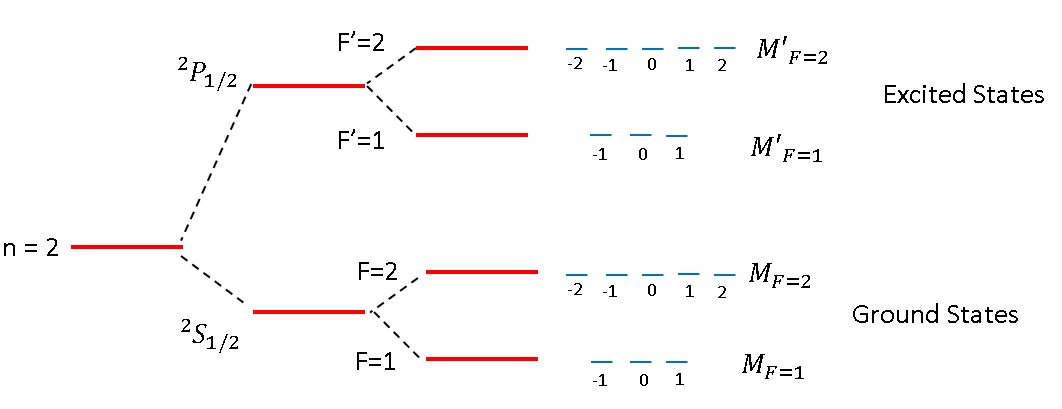
\includegraphics[width = 0.8\textwidth]{fig1}
  \label{fig1}
\end{figure}

\subsection{Aim and importance of this work}
In this work, I'm simulating the optical pumping process of the D1 line of lithium 7 atoms. In the lab, we are using this optical puming process to detect lithium atom signal in the vacuum chamber. While normal fluorescence imaging using a single resonant laser can do the detection job, optical pumping can allow us to detect much weaker $^{7}Li$ signals, especially the total atoms number to be detected is small. \\

Basically we want to transfer all atoms from ground state $F=1$ to ground state $F=2, M_f = 2$. However, experimently there are two possible transitions for us to chose for the optical pumping, as shown in fig \ref{fig2}. \\ % add fig here
\begin{figure}[!h]
  \centering
  \caption{}
  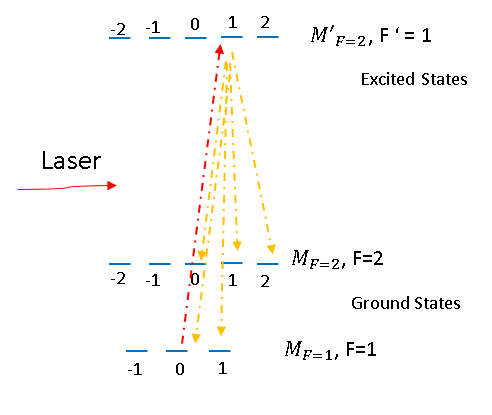
\includegraphics[width = 0.5\textwidth]{fig2}
  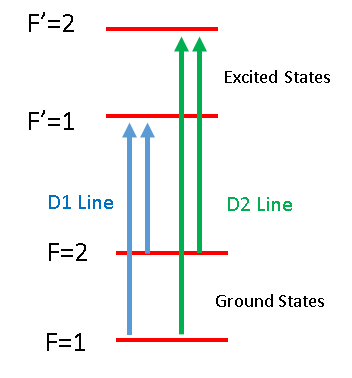
\includegraphics[width = 0.4\textwidth]{fig4}
  \label{fig2}
\end{figure}

One is to use excited state $F\prime = 1$ as the medium, which has 3 magnetic sublevels: $M_F = -1, 0, 1$, another choice is to use excited state $F\prime = 2$, which has 5 magnetic sublevels: $M_F = -2, -1, 0, 1, 2$. \\

In this simulation, I will compare the two different optical pumping schemas under same physics condition, to figure out which schema will lead to a faster optical pumping trnasition. The result will be used to guid our fellowing experiment. 

\section{Project}
In this section, I'll show the serial code structure to introduce how the simulation works. Based on this, I'll discuss the approach of parallelizing the code and the reason I'm doing it in this way. By the end I'll shown the performance of the parallelized code. \\
The project is done with C++, parallized by OpenMP, result plotted by python. 
\subsection{Code structure}
The code structure is shown is fig \ref{fig5}. \\ 
% add picture here
\begin{figure}[h]
  \centering
  \caption{}
  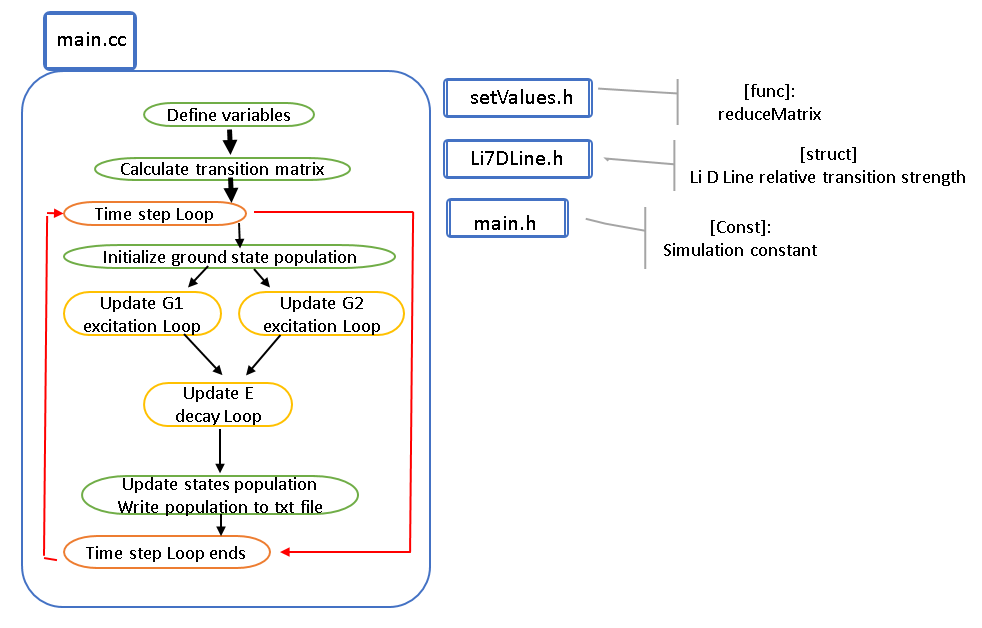
\includegraphics[width = 0.8\textwidth]{fig5}
  \label{fig5}
\end{figure}

The simulation is made of 4 parts:
\begin{enumerate}
\item Generate transition matrix
\item Initialize ground states population
\item Simulate excitation process for the 2 ground states
\item Simulate decay process from excited states to 2 ground states
\item Calculate the new population for the 2 gound states and excited state write data to file
\item Loop the above two steps for giving time (number of loops)
\item Generate plot for population of different states versus time
\end{enumerate}


\subsection{Parallelization}
There are multiple loops in the code, so considering using OpenMP to parallelize some of them. \\
Only considering those big loops that under goes lots of computation, find that there are potentially 4 loops that worth being parallized:
\begin{enumerate}
\item General time step loop. This could have hundreds of thoustands of iterations.
\item Update ground state G1 loop. This has 3 loops, but each loop may have heavy computation work.
\item Update ground state G2 loop. This has 3 loops, but each loop may have heavy computation work.
\item Update Excited state E loop. This also requires a lot of computation.
\end{enumerate}
Now I'm going to analyze the possiblity to parallelize each of above loops:\\

For 1,  physics of optical pumping requires that each of time step iterations depend on the previous iteration, since that's the results of previous iteration becomes the starting state of the coming iteration. For this reason, unfortunately, this biggest loop cannot be parallelized due to the  indepedency of each iteration.\\

For 2, 3, although this two loop are with the time iteration loop, they have independency of each iterations, the computation of excitation process for the two ground states doesn't depent on the population of the magnetic sublevels (iterations). Further more these two loop are computation intensive, since each of the iterations has to do a big matrix multiply calculation. Based on these facts, this  two loops should be parallelized.\\

For 4, this is similar to loop 2 and loop 3, in terms of the independency and calculation intensity. However, this loop has to be excuted after the two loop, since one has to check if the loop 2 and loop 3 have already depleted the ground states, the uptating algorithm for this loop depend on loop 2 and loop 3. This is in consideration of the conservation of atoms number (In this simulation, I'm using number density, so total atom number should always be 1, when sum up each of the substates). Based on these facts, this loop can be prarllelized, but it must be excuted after the previous two loops.\\

Overall, I decide to parallel the loop 2,3,and 4, while keep the loop 4 excuted after loop 2 and 3. Considering there are only 3 and 5 interations in loop 2 and loop 3, I decide to let each of these 2 loops excute in parallel but each on one thread. For loop 3, which has 5 calculation intensive iterations, I would assign 5 threads to parallelizd this region. The diagram for the prarllization as shown in fig \ref{fig6}: \\

\begin{figure}[h]
  \centering
  \caption{}
  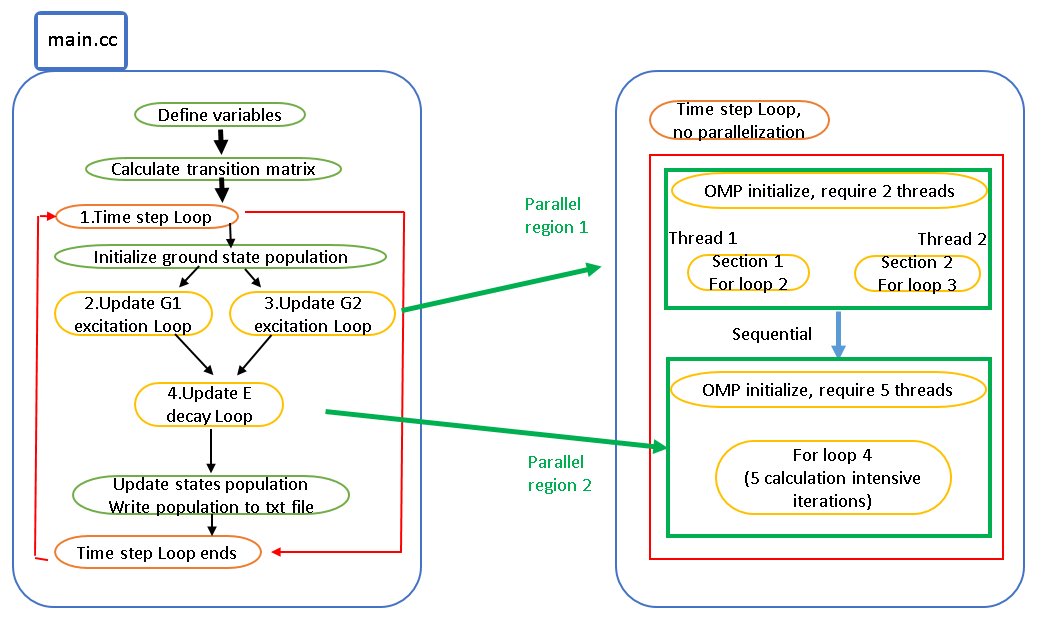
\includegraphics[width = 0.8\textwidth]{fig6}
  \label{fig6}
\end{figure}


\section{Result and discussion}
By using the parallized code, I simulated the 2 optical pumping schemas: use $F\prime = 1$ as excited state and use $F\prime = 2$ as excited state. Here I'll show one of the comparision under the same physics condition.

\subsection{$F\prime = 1$as excited state}
See figure \ref{fig7}\\
\begin{figure}[h]
  \centering
  \caption{}
  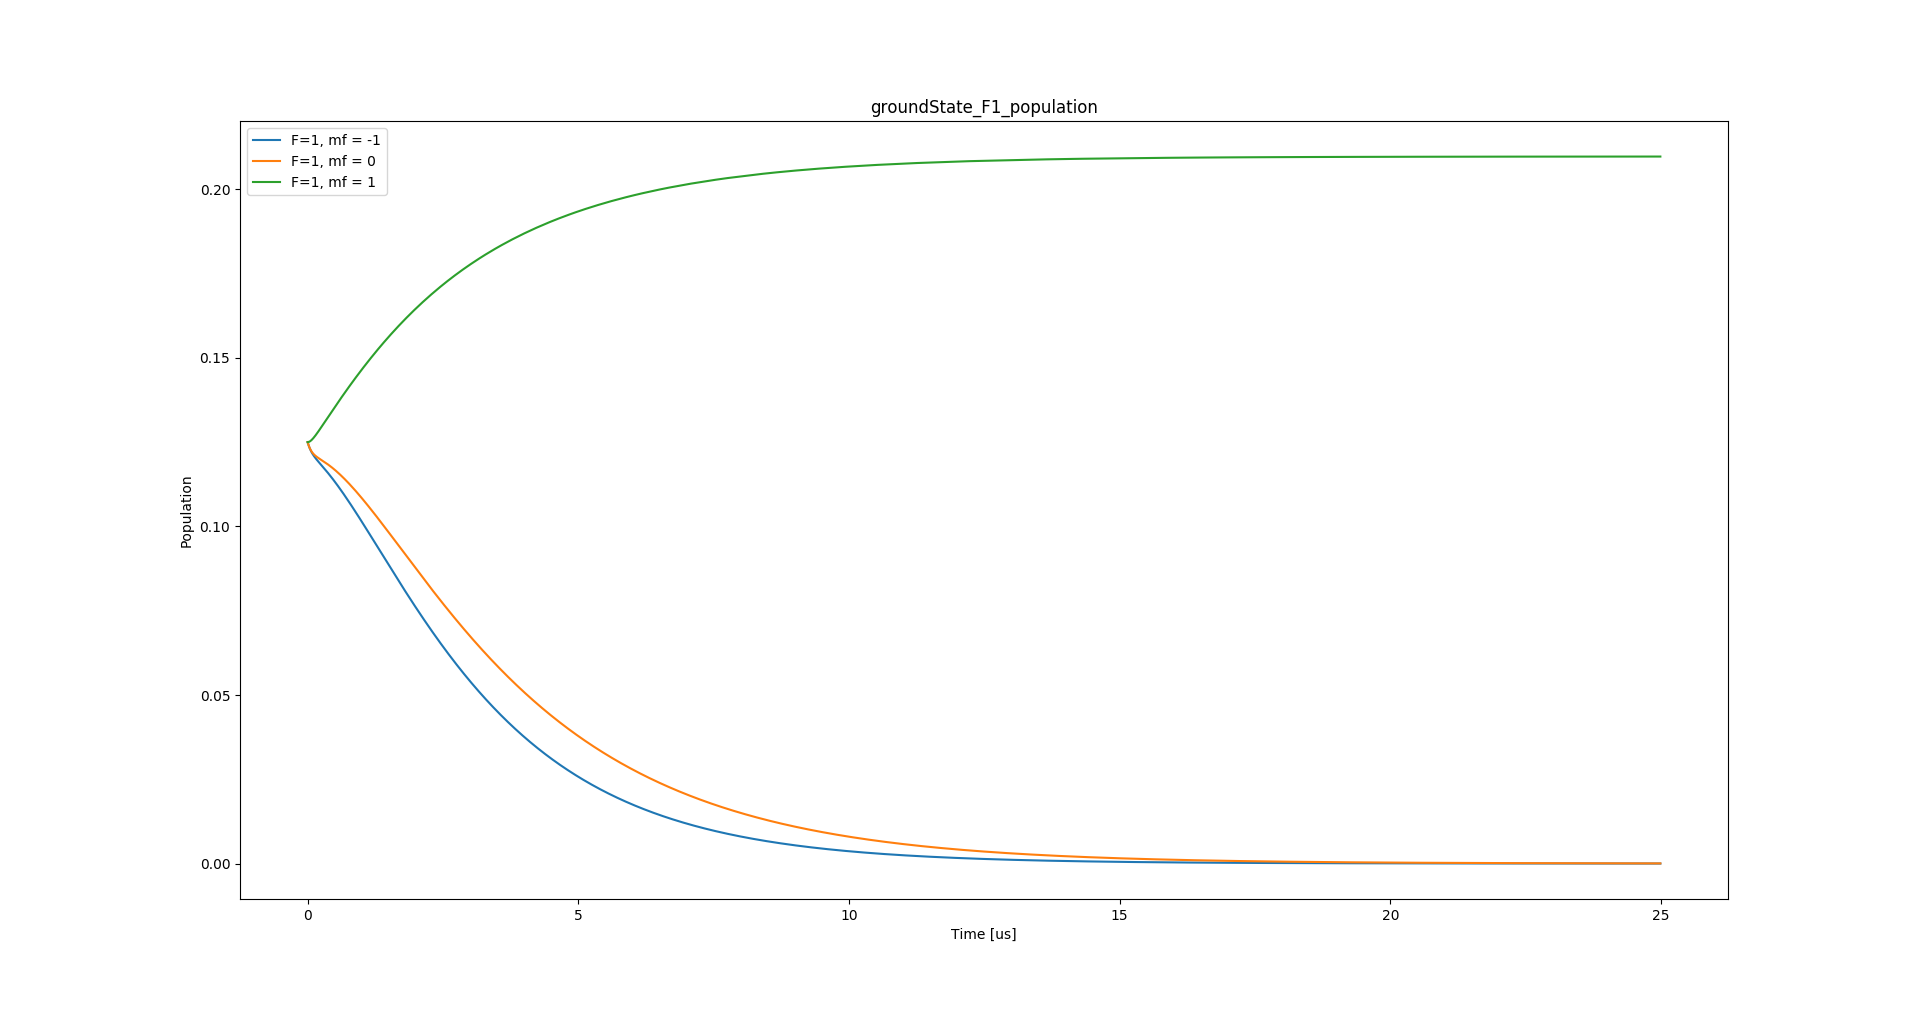
\includegraphics[width = 1.15\textwidth]{f1fig1}
  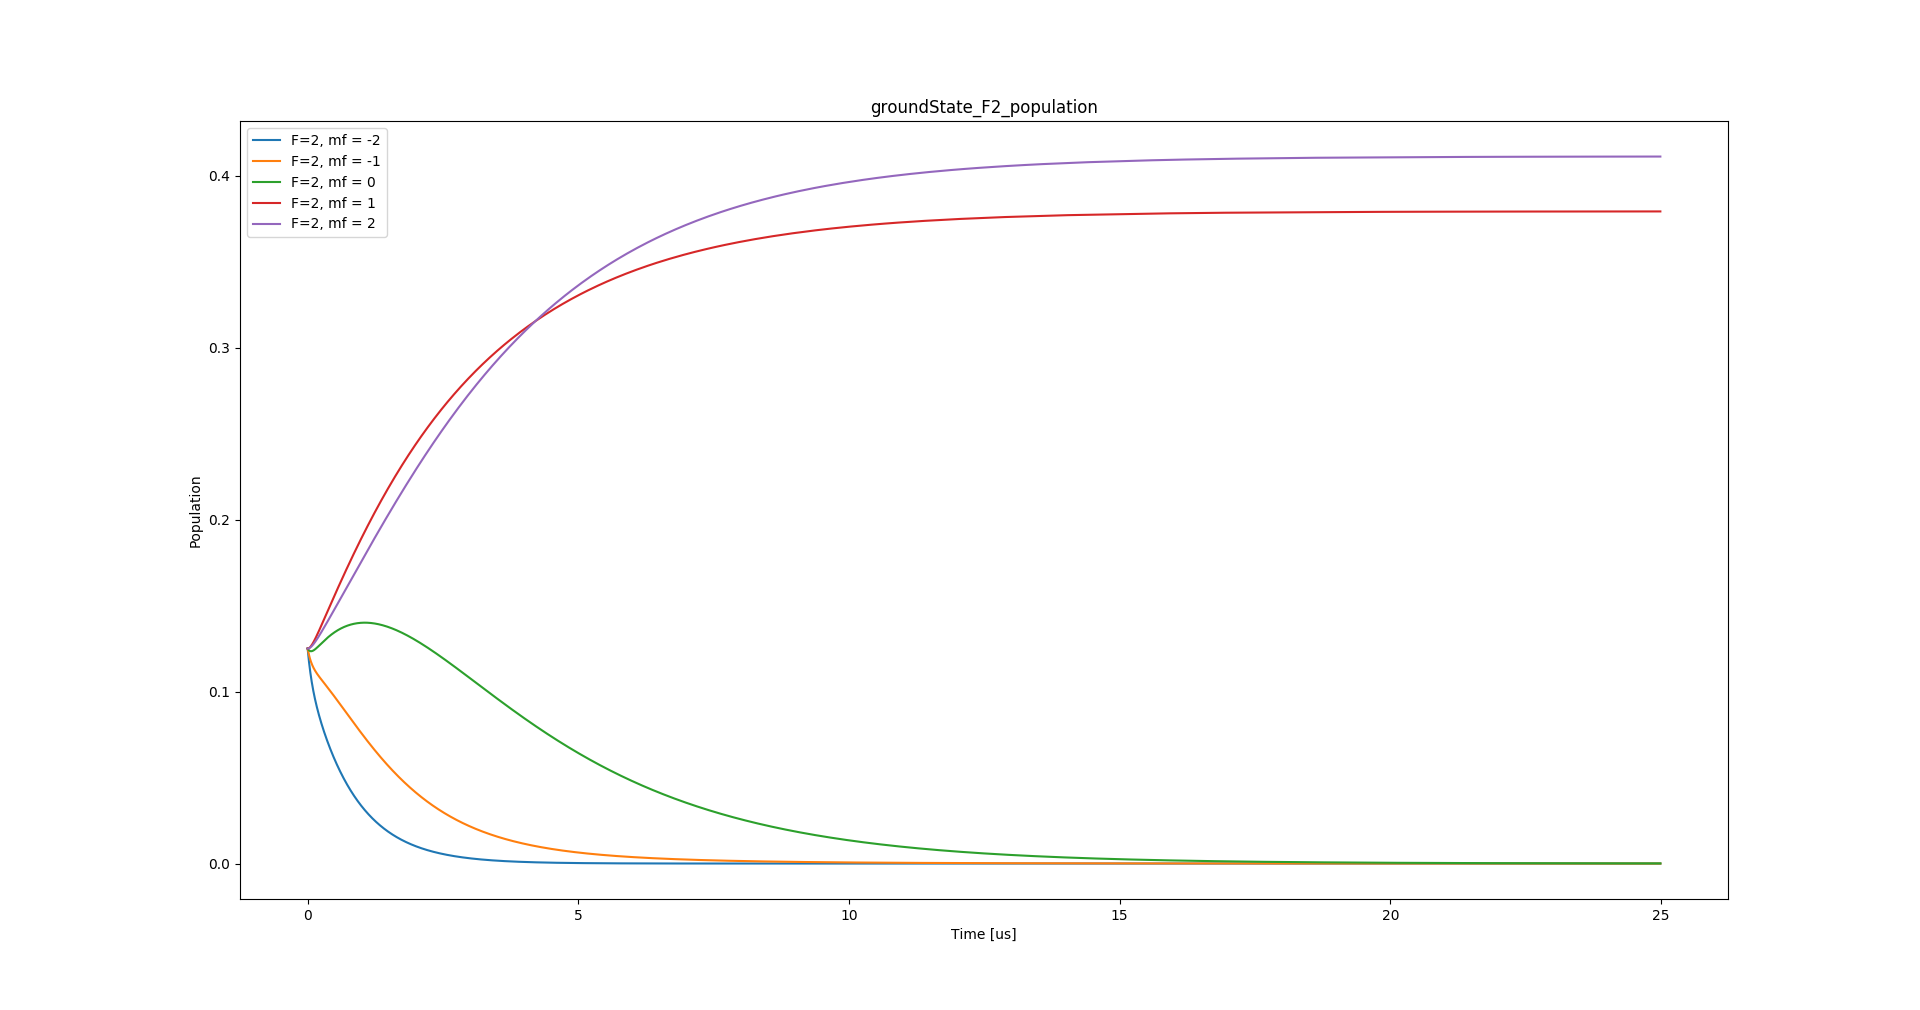
\includegraphics[width = 1.15\textwidth]{f1fig2}
  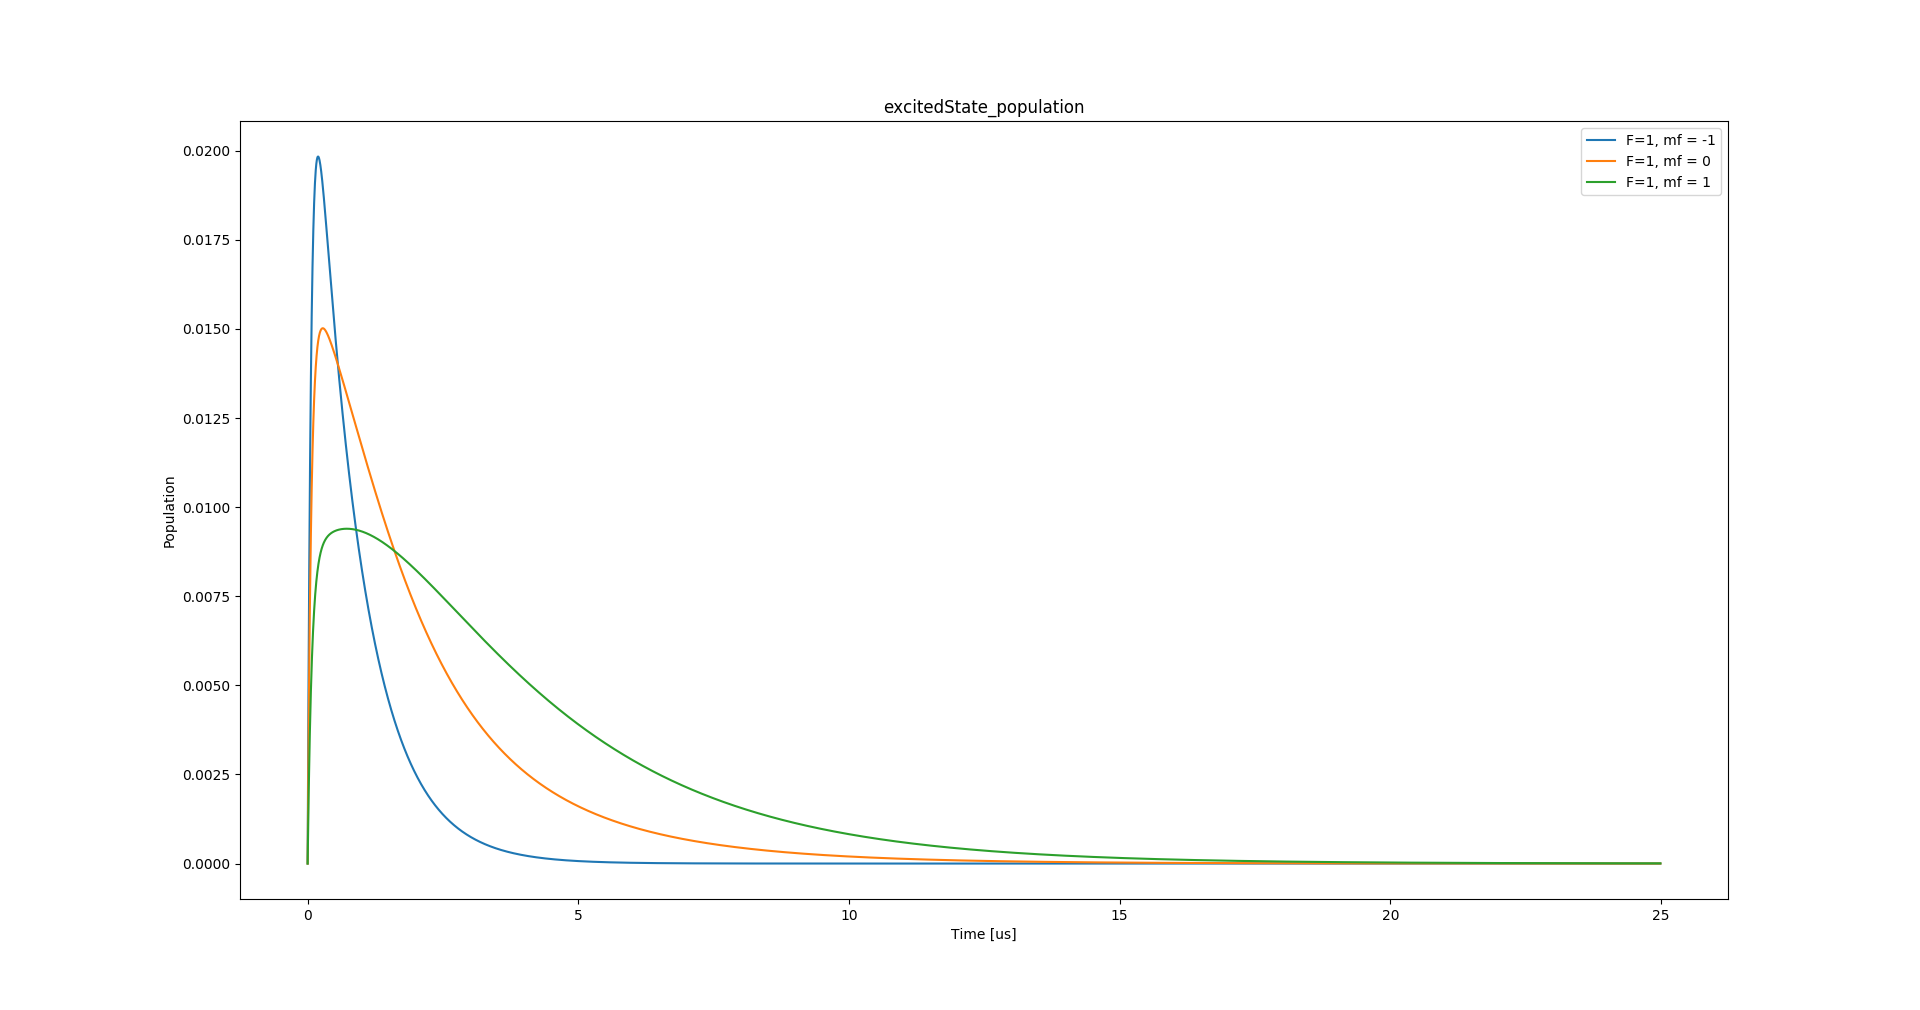
\includegraphics[width = 1.15\textwidth]{f1fig3}
  \label{fig7}
\end{figure}



\subsection{$F\prime = 2$as excited state}
See figure \ref{fig8}\\
\begin{figure}[h]
  \centering
  \caption{}
  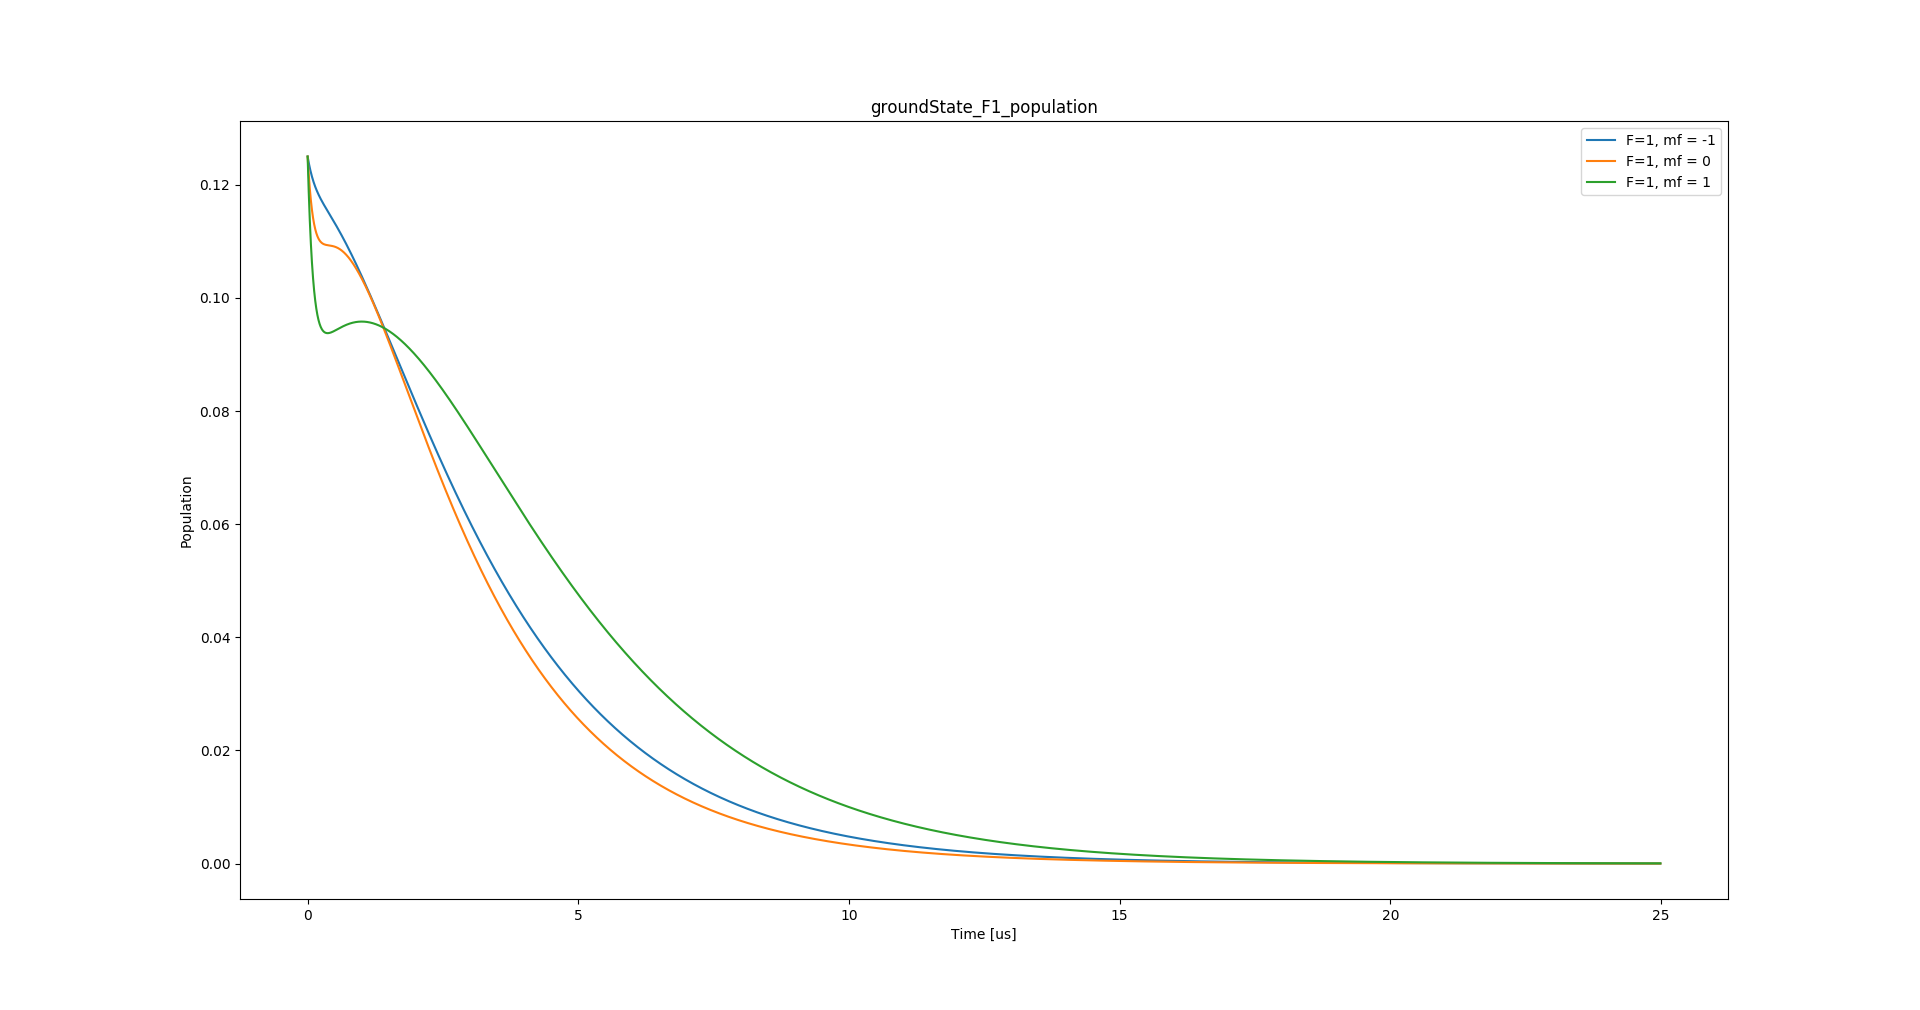
\includegraphics[width = 1.15\textwidth]{f2fig1}
  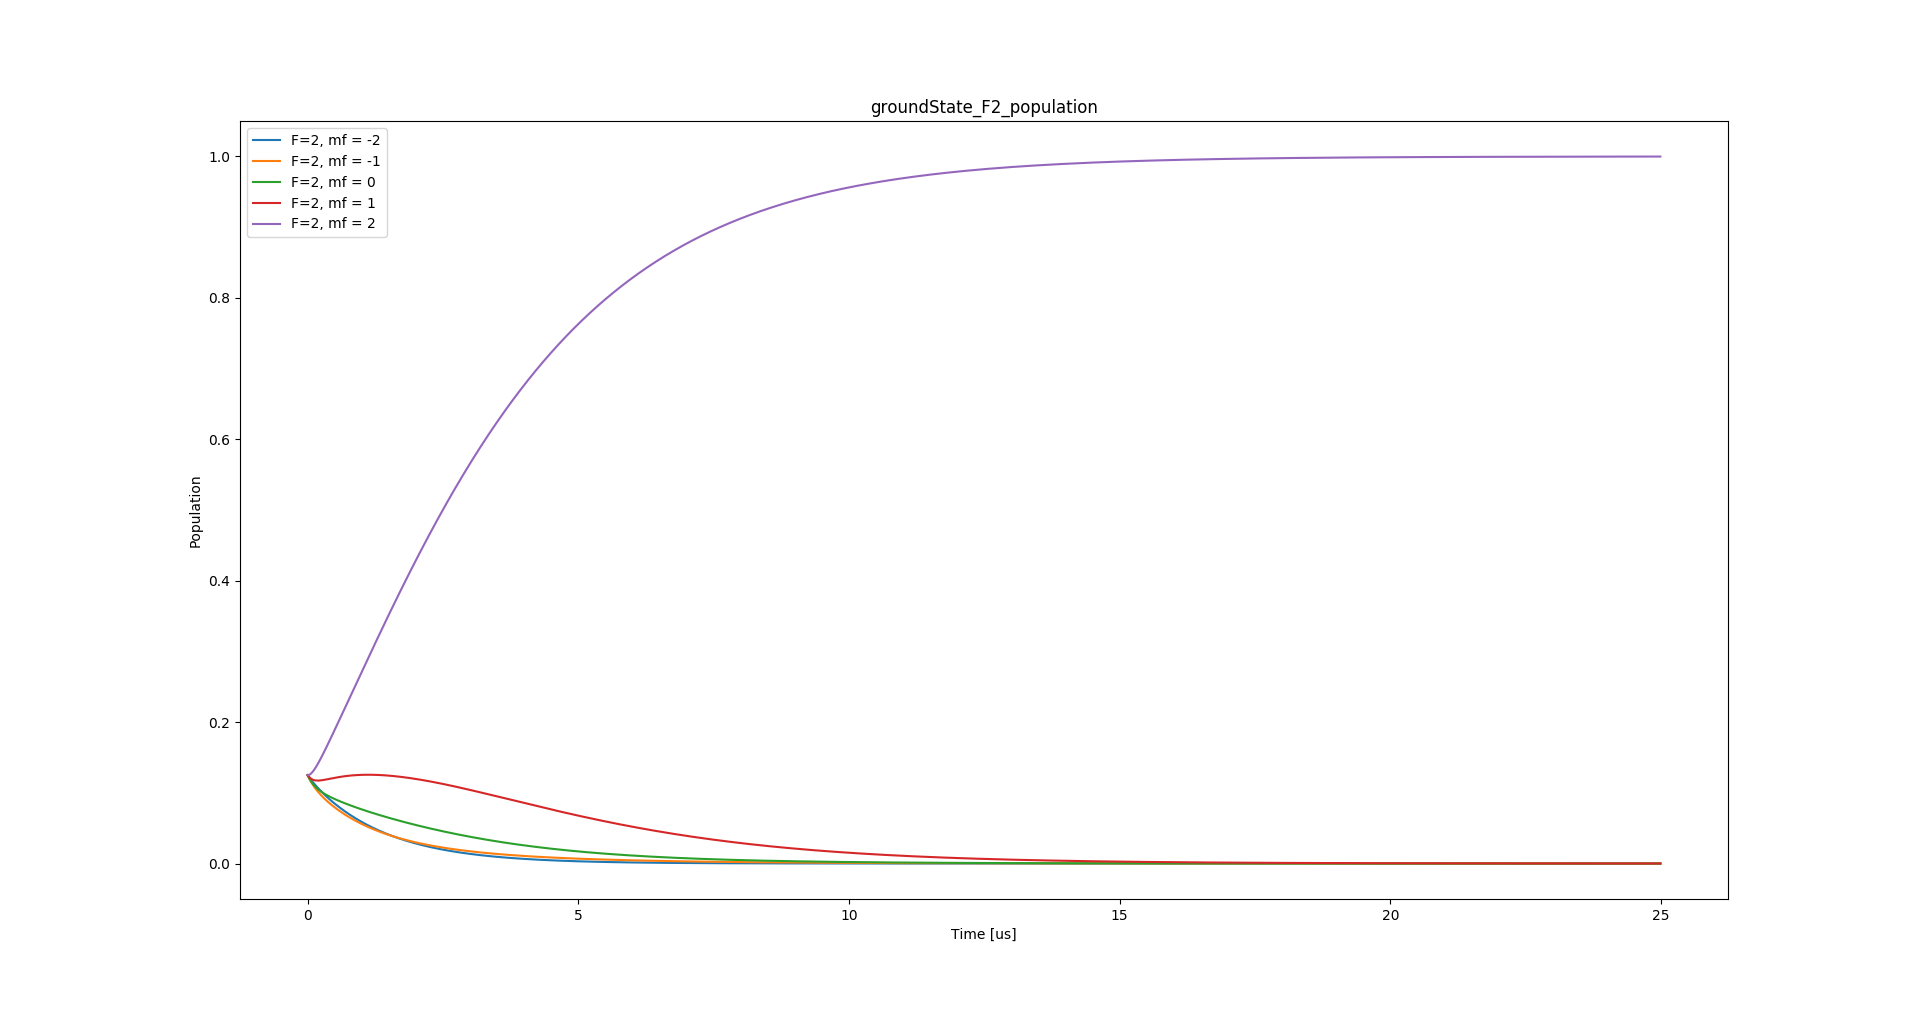
\includegraphics[width = 1.15\textwidth]{f2fig2}
  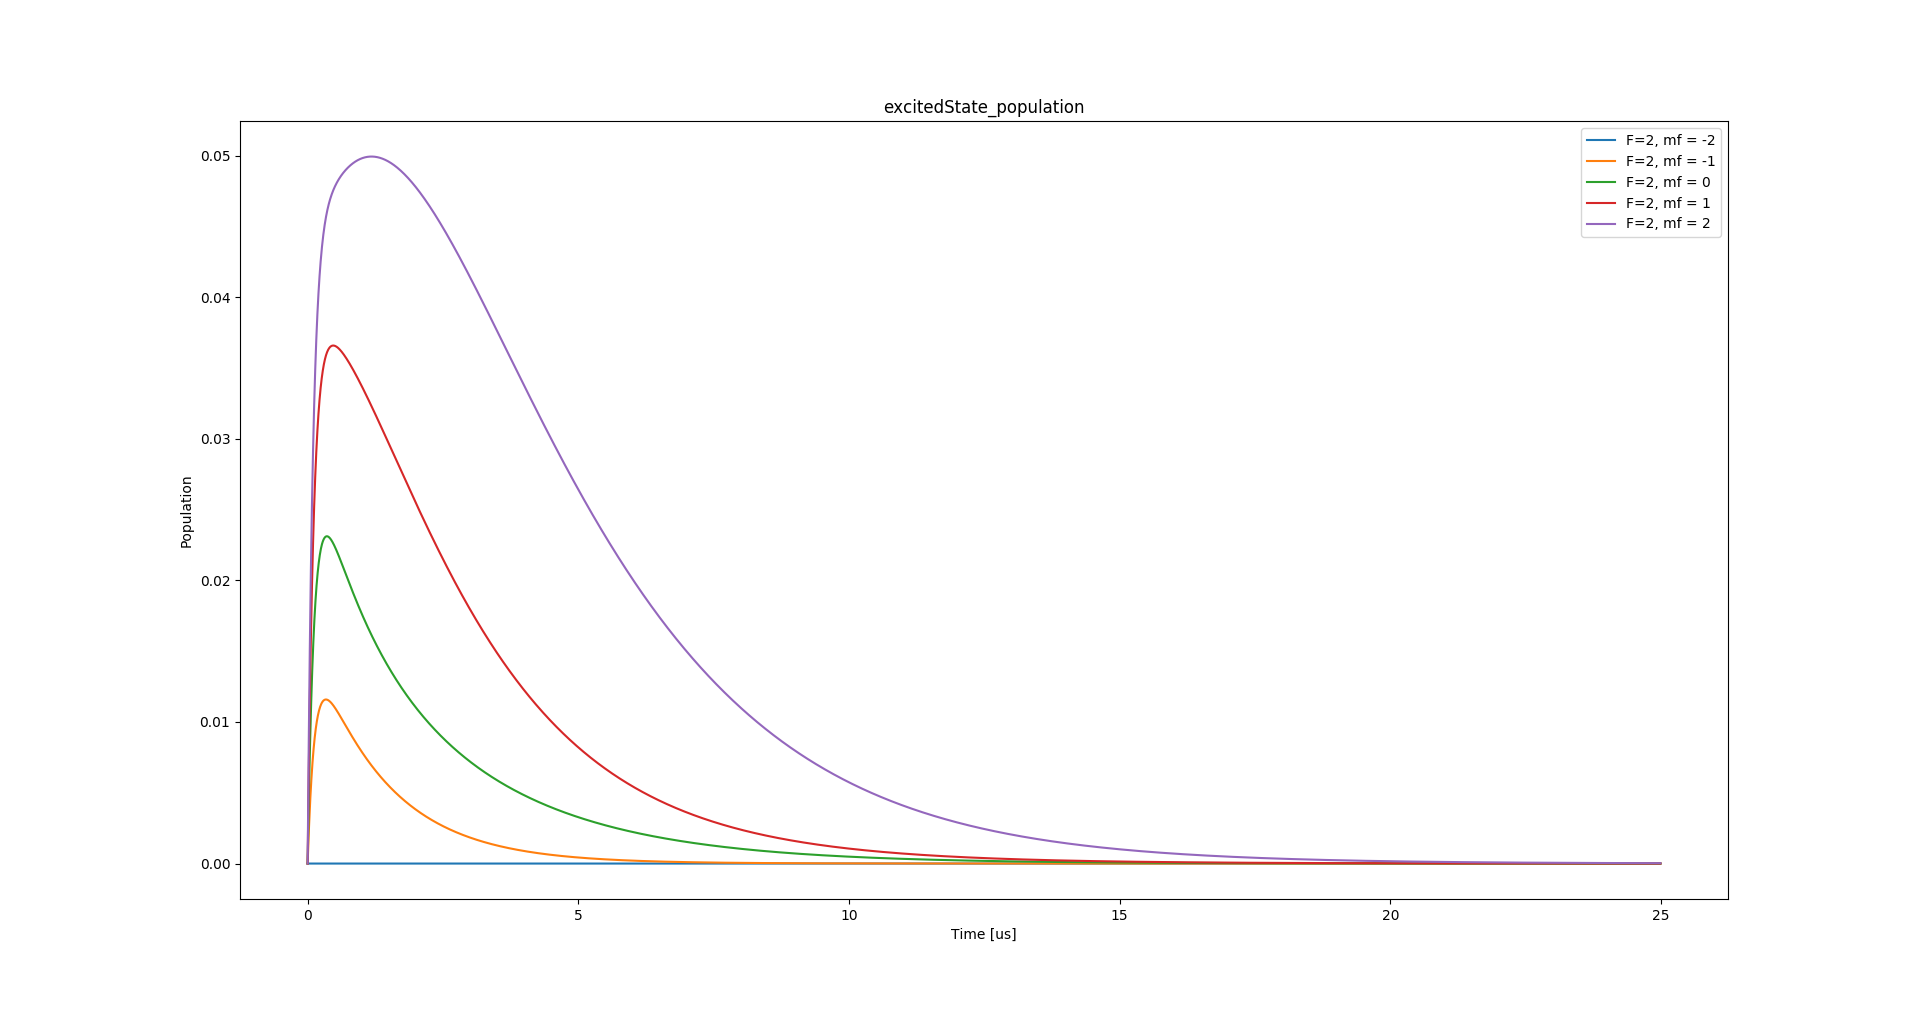
\includegraphics[width = 1.15\textwidth]{f2fig3}
  \label{fig8}
\end{figure}

\subsection{Discussion}
From the plot, one can see that, if choose $F\prime = 1$ as excited state to do the optical pumping, we cannot transfer all of the population to a single state, while we can achieve this goal by chosing $F\prime = 2$ as excited state.  while in terms of the time to reach a stable state, both of these to schema take about the same time. Since pump the atom into a single state is very important for our experiment, based on this simulation, we will chose $F\prime = 2$ as the excited state to do the optical pumping.

\section{Summary}
To sum up, starting from a pratical physics problem, simulation code was written, as a step further, the chose of Parallelization was discussed and realized by using OpenMp. The simulation results were discussed and come to a conclusion to help guide the experiment. 
\pagenumbering{gobble} 

  
\end{document}